\chapter{Ejercicio Práctico N.º 1: Tareas y Planificación}
\label{sec.ej1:planificacion}

\section{Descripción General}

El primer ejercicio tiene como propósito implementar un esquema de multitarea apropiativa
utilizando el núcleo de FreeRTOS, verificando la coexistencia de múltiples flujos de ejecución concurrentes con
diferentes niveles de prioridad y períodos de repetición.

El sistema debe ejecutar de forma simultánea tres actividades con restricciones temporales diferenciadas:
el parpadeo de un LED de señalización a frecuencia constante, la emisión periódica de una cadena de texto con datos
de diagnóstico a través del puerto serie USART1, y el cómputo de la disponibilidad de procesamiento mediante el monitoreo
de la tarea Idle.

\section{Estructura de Tareas y Prioridades}

Para satisfacer las consignas se definieron dos tareas de usuario explícitas y se habilitó la función \textit{IdleHook}
asociada a la tarea del sistema. En la tabla \ref{tab.ej1:tareas} se resumen los parámetros de configuración
asignados a cada tarea durante la inicialización.

\begin{table}[!ht]
\centering
\small
\caption{Parámetros de configuración de las tareas en el Ejercicio 1.}
\label{tab.ej1:tareas}
\begin{tabular}{llcccl}
\toprule
Tarea & Función & Prioridad & Stack & Período & Salida / Acción \\
\midrule
Tarea A & \texttt{vBlink} & 3 & 256 pal. & $\SI{100}{\milli\second}$ & Pin PC13 (LED) \\
Tarea B & \texttt{vSendTelemetry} & 2 & 256 pal. & $\SI{2000}{\milli\second}$ & USART1 (PA9) \\
Tarea C & \texttt{IdleHook} & 0 & Stack Idle & Continuo & Incremento de \texttt{ulIdleCount} \\
\bottomrule
\end{tabular}
\end{table}

La jerarquía de prioridades adoptada responde a los criterios fundamentales de los sistemas de tiempo real:

\begin{enumerate}
  \item \textbf{Tarea A (\texttt{vBlink}, prioridad 3)}: Se le asigna la prioridad más alta entre las tareas de usuario
    a fin de asegurar que el cambio de estado lógico en el pin PC13 no sufra fluctuaciones temporales inducidas
    por la actividad de comunicaciones serie. El período de conmutación se fijó en $\SI{100}{\milli\second}$, lo que
    determina un ciclo completo de encendido y apagado de $\SI{200}{\milli\second}$, cumpliendo con la frecuencia de
    parpadeo de $\SI{5}{\hertz}$.
  \item \textbf{Tarea B (\texttt{vSendTelemetry}, prioridad 2)}: Posee una prioridad intermedia. Se ejecuta una vez cada
    $\SI{2000}{\milli\second}$ ($\SI{2}{\second}$) para componer una cadena de texto en memoria y transmitirla byte a
    byte mediante el periférico USART1. Al disponer de menor prioridad que la Tarea A, si el temporizador de
    $\SI{100}{\milli\second}$ expira mientras la Tarea B está enviando datos, el planificador suspende su ejecución ,
    atiende el cambio de estado del LED y reanuda la transmisión serie.
  \item \textbf{Tarea C (\texttt{Idle Hook}, prioridad 0)}: La tarea de inactividad es instanciada internamente por
    FreeRTOS con la prioridad más baja del sistema. Ejecuta la función \texttt{vApplicationIdleHook()} únicamente cuando
    las tareas A y B se encuentran bloqueadas a la espera del vencimiento de sus respectivos intervalos de retardo.
\end{enumerate}

En la figura \ref{fig.ej1:cronograma} se ilustra el cronograma temporal del sistema y la dinámica de desalojo
conducida por el planificador del kernel.

\begin{figure}[!ht]
\centering
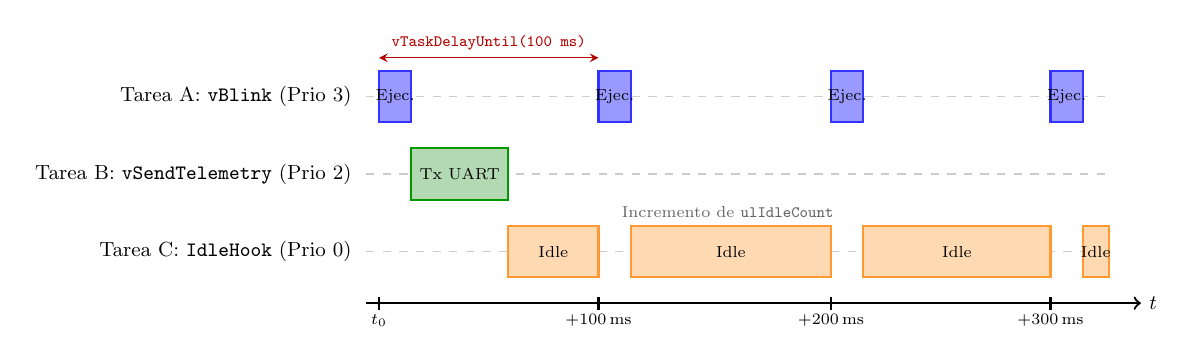
\begin{tikzpicture}[scale=0.82, transform shape, every node/.style={font=\small}]
  % Ejes de tareas
  \draw[->, thick] (0,0) -- (12,0) node[right] {$t$};
  \node[left] at (-0.1, 3.2) {Tarea A: \texttt{vBlink} (Prio 3)};
  \node[left] at (-0.1, 2.0) {Tarea B: \texttt{vSendTelemetry} (Prio 2)};
  \node[left] at (-0.1, 0.8) {Tarea C: \texttt{IdleHook} (Prio 0)};

  % Líneas base
  \draw[gray!40, dashed] (0, 3.2) -- (11.5, 3.2);
  \draw[gray!40, dashed] (0, 2.0) -- (11.5, 2.0);
  \draw[gray!40, dashed] (0, 0.8) -- (11.5, 0.8);

  % Tarea A (vBlink) - se ejecuta periódicamente cada 100 ms (pulsos breves)
  \fill[blue!40, draw=blue!80, thick] (0.2, 2.8) rectangle (0.7, 3.6) node[pos=0.5, black, font=\scriptsize] {Ejec.};
  \fill[blue!40, draw=blue!80, thick] (3.6, 2.8) rectangle (4.1, 3.6) node[pos=0.5, black, font=\scriptsize] {Ejec.};
  \fill[blue!40, draw=blue!80, thick] (7.2, 2.8) rectangle (7.7, 3.6) node[pos=0.5, black, font=\scriptsize] {Ejec.};
  \fill[blue!40, draw=blue!80, thick] (10.6, 2.8) rectangle (11.1, 3.6) node[pos=0.5, black, font=\scriptsize] {Ejec.};

  % Tarea B (vSendTelemetry) - ejecuta al inicio o cada 2 s, es desalojada o corre tras Tarea A
  \fill[green!50!black!30, draw=green!60!black, thick] (0.7, 1.6) rectangle (2.2, 2.4) 
    node[pos=0.5, black, font=\scriptsize] {Tx UART};

  % Tarea C (Idle Hook) - corre en todo el tiempo restante
  \fill[orange!30, draw=orange!80, thick] (2.2, 0.4) rectangle (3.6, 1.2) node[pos=0.5, black, font=\scriptsize] {Idle};
  \fill[orange!30, draw=orange!80, thick] (4.1, 0.4) rectangle (7.2, 1.2) node[pos=0.5, black, font=\scriptsize] {Idle};
  \fill[orange!30, draw=orange!80, thick] (7.7, 0.4) rectangle (10.6, 1.2) node[pos=0.5, black, font=\scriptsize] {Idle};
  \fill[orange!30, draw=orange!80, thick] (11.1, 0.4) rectangle (11.5, 1.2) node[pos=0.5, black, font=\scriptsize] {Idle};

  % Marcadores temporales
  \draw[thick] (0.2, -0.1) -- (0.2, 0.1) node[below=4pt, font=\scriptsize] {$t_0$};
  \draw[thick] (3.6, -0.1) -- (3.6, 0.1) node[below=4pt, font=\scriptsize] {$+100\,\mathrm{ms}$};
  \draw[thick] (7.2, -0.1) -- (7.2, 0.1) node[below=4pt, font=\scriptsize] {$+200\,\mathrm{ms}$};
  \draw[thick] (10.6, -0.1) -- (10.6, 0.1) node[below=4pt, font=\scriptsize] {$+300\,\mathrm{ms}$};

  % Flechas y anotaciones
  \draw[<->, >=stealth, red!70!black] (0.2, 3.8) -- (3.6, 3.8) 
    node[midway, above, font=\scriptsize] {\texttt{vTaskDelayUntil(100 ms)}};
  \node[above, font=\scriptsize, gray!80!black] at (5.6, 1.2) {Incremento de \texttt{ulIdleCount}};
\end{tikzpicture}

\caption{Cronograma de ejecución y asignación de CPU entre tareas en el Ejercicio 1.}
\label{fig.ej1:cronograma}
\end{figure}

\section{Recursos de FreeRTOS Utilizados}
\label{sec.ej1:recursos}

El funcionamiento del programa se apoya en los siguientes servicios y primitivas provistos por el kernel:

\subsection{Creación e Inicialización de Tareas}

\begin{lstlisting}[language=C]
res = xTaskCreate(vBlink, "Blink", 256, NULL, 3, NULL);
if (res != pdPASS) {
    while(1);
}
\end{lstlisting}

Se verifica sistemáticamente el valor de retorno. Si la función retorna un código distinto de \texttt{pdPASS}, se
detiene el flujo de ejecución en una condición segura de error.

Una vez configuradas las tareas y los periféricos de hardware mediante llamadas a registros CMSIS, la llamada a
\texttt{vTaskStartScheduler()} inicializa el temporizador SysTick a una cadencia de $\SI{1000}{\hertz}$
(\texttt{configTICK\_RATE\_HZ = 1000}) e inicia la ejecución de la tarea de mayor prioridad lista.

\subsection{Temporización Determinística con \texttt{vTaskDelayUntil}}

Para garantizar una periodicidad rigurosa sin acumulación de corrimiento temporal, se optó por el uso de
\texttt{vTaskDelayUntil()} en lugar de la función de retardo relativo convencional \texttt{vTaskDelay()}.

\begin{lstlisting}[language=C]
void vBlink(void *pvParameters) {
    TickType_t xLastTickEntry = xTaskGetTickCount();
    while (1) {
        GPIOC->ODR ^= GPIO_ODR_ODR13;
        vTaskDelayUntil(&xLastTickEntry, pdMS_TO_TICKS(100));
    }
}
\end{lstlisting}

La función toma como referencia el valor absoluto del conteo de ticks capturado al inicio (\texttt{xLastTickEntry})
y calcula internamente el instante exacto del siguiente desbloqueo sumando el número de ticks equivalente a
$\SI{100}{\milli\second}$ (\texttt{pdMS\_TO\_TICKS(100)}). De este modo, las fluctuaciones en el tiempo de
la ejecución del cuerpo del bucle no alteran el periodo global de repetición.

\subsection{Monitoreo de Carga con la Función Idle Hook}

En el archivo de configuración del kernel se estableció la directiva \texttt{configUSE\_IDLE\_HOOK = 1}. Bajo esta
condición, cada vez que la tarea Idle toma el procesador, invoca a la función de retorno definida por la aplicación:

\begin{lstlisting}[language=C]
void vApplicationIdleHook(void) {
    ulIdleCount++;
}
\end{lstlisting}

La variable \texttt{ulIdleCount} se declara como volátil (\texttt{volatile uint32\_t}) para evitar que el compilador
optimice su acceso en registros de CPU. En cada ciclo de telemetría ($\SI{2}{\second}$), la Tarea B formatea el valor
acumulado en dicha variable y lo transmite:

\begin{lstlisting}[language=C]
uint32_t length = sprintf(buffer, "%s%lu\r\n", string, ulIdleCount);
for (uint16_t i = 0; i < length; i++) {
    while ((USART1->SR & USART_SR_TXE) == 0);
    USART1->DR = buffer[i];
}
\end{lstlisting}

La velocidad de incremento de este contador permite corroborar que el microcontrolador permanece la mayor parte del
tiempo disponible en estado inactivo, dado que la Tarea A solo utiliza unos pocos microsegundos por ciclo para conmutar
el bit en el registro \texttt{GPIOC->ODR} y la Tarea B interviene únicamente una vez cada dos segundos.
